\chapter{Data}\label{sec:data}
To answer the research question, we used the DevGPT dataset~\cite{devgpt}, which contains \acrshort{gpt} conversations shared on GitHub and Hacker News between late May 2023 and October 12, 2023. The dataset includes nine snapshots (latest: October 12, 2023), each comprising links to \acrshort{gpt} conversations found in GitHub commits, issues, discussions, pull requests, code files, and Hacker News articles. Considering the origins the conversations were sourced from, it is safe to assume that the prompts for this conversations were written by software developers.

In this study, we use data from all available snapshots. To ensure data quality, we removed duplicate entries based on shared \acrshort{gpt} conversation links. Additionally, we extended the DevGPT dataset with a new dataset collected in March 202. This extension contains developer-chatbot conversations shared in the same sources but posted after the latest DevGPT snapshot. The structure of the extended dataset mirrors that of DevGPT to maintain consistency. The dataset was provided for this research by author's colleagues from the same research group.

Table~\ref{table:data_stat} presents the number of unique conversations sourced from each data source, along with the remaining number of conversations after removing duplicates and non-English conversations.

\begin{table}[h]
    \centering
    \resizebox{\textwidth}{!}{%
    \begin{tabular}{|l|c|c|c|c|c|c|c||c|}
        \hline
        & Commits & Issues & Discussions & Pull req. & Code files & Repositories & Hacker News & Total \\
        \hline
        \hline
        DevGPT DR & 670 & 516 & 59 & 268 & 2010 & 0 & 322 & 3845\\
        \hline
        Extension DR & 881 & 1134 & 65 & 775 & 9536 & 10 & 805 & 13206 \\
        \hline
        Combined DR & 896 & 1235 & 113 & 813 & 9959 & 10 & 858 & 13884 \\
        \hline
        Combined NE & 862 & 998 & 89 & 682 & 8057 & 8 & 773 & 11469 \\
        \hline
    \end{tabular}
    }
    \caption{Number of conversations collected from different sources after all the duplicates (DR) and non-English conversations (NE) were removed from the data.}
    \label{table:data_stat}
\end{table}

The total number of conversations shared across all the sources after duplicates and non-English conversations were removed is 11469. However, after removing duplicate conversations from the entire combined dataset, it leaves us with 10279 conversations, which means that 1190 \linebreak developer-\acrshort{gpt} conversations are shared in multiple locations.

\section{Data cleaning}
During our initial analysis of the dataset, we identified the presence of information irrelevant to the research question --- referred to as ``noise''. First, many prompts contain embedded code alongside natural language. A good example of this is the following prompt from DevGPT dataset sourced from GitHub Issues: 

\textit{So you want me to hard code the password in this section of src/pages/\linebreak api/getDeviceInfo.js?}
\begin{fleqn}
\begin{flalign*}
const \ &pool = new \ Pool(\{ \\
&host: process.env.PGHOST\_2,\\
&port: process.env.PGPORT\_2,\\
&database: process.env.PGDATABASE\_2,\\
&user: process.env.PGUSER\_2,\\
\});
\end{flalign*}
\end{fleqn}

Second, while we focus exclusively on English-language conversations, the dataset includes interactions in multiple languages. For example, the following prompts was sourced from conversation shared in GitHub commits: \textit{mach mir noch so eine aufgabe zu dem selben muster, damit ich das thema besser verstehen kann}. 

Both of the mentioned factors introduce noise that must be removed before proceeding with data exploration and answering the research questions.

\subsection{Code detection and its accuracy}\label{sec:prog-identification}
Initially we attempted to detect programming language content using the Guesslang Python library\footnote{\url{https://pypi.org/project/guesslang/}}, but its accuracy and F1-score were too low for our dataset. As a result, we developed a custom method for identifying and filtering out programming lines.

To identify code segments within prompts, we first split each prompt into individual lines using the line break character (\textit{\textbackslash n}). We then applied a custom script to estimate the likelihood that each line contains code. This approach is based on the assumption that code blocks typically appear on separate lines from natural language text and often span multiple lines within a prompt. As a result, line-by-line analysis is necessary to accurately detect code.

To identify whether a line is written in a programming language or natural language, we implemented a function that evaluates the line’s structures --- whether they are tokens or full sentences --- and assigns them a probability score: \texttt{0} indicates a programming language structure, \texttt{0.5} indicates ambiguity (could be either), and \texttt{1} indicates natural language. The list below shows what kind of structures are considered in this script:
\begin{itemize}
    \item Line is empty (likelihood: 0);
    \item Line starts a multiline comment block with symbols like \texttt{/*}, \texttt{"""}, \texttt{'''}, or \texttt{<!--}, and does not end on the same line --- the whole block is marked as comment (likelihood: 0);
    \item Line is within a multiline comment block and ends with symbols like \texttt{*/}, \texttt{"""}, \texttt{'''}, or \texttt{-->} --- marked as comment (likelihood: 0);
    \item Line matches single-line comment patterns such as \texttt{//}, \texttt{\#}, \texttt{--}, etc. --- marked as comment (likelihood: 0);
    \item Line starts with an opening HTML tag (e.g. \texttt{<div>}) and does not end with a closing tag --- line and subsequent lines until closing tag are marked as HTML (likelihood: 0);
    \item Line contains a complete HTML block (e.g. \texttt{<p>Text</p>}) --- marked as HTML (likelihood: 0);
    \item Line is tokenized using \texttt{shlex.split} if it contains quotes, otherwise by whitespace. Each token (word) is assigned a probability score based on specific heuristics:
    \begin{itemize}
        \item Word contains space and resembles a sentence --- averaged likelihood from subword analysis;
        \item Word starts with tab (likelihood: 0);
        \item Word is in a list of known programming keywords (likelihood: 0.5);
        \item Word is a camelCase or PascalCase identifier (likelihood: 0);
        \item Word is in UPPERCASE (e.g. SQL keywords; likelihood: 0.5);
        \item Word is purely alphabetical (likelihood: 1);
        \item Word is a comment-like or inline programming pattern (e.g. \texttt{::}, \texttt{\#}, \texttt{<\textbackslash }, \texttt{<|-};  likelihood: 0);
        \item Word matches function calls, method chains, array indexing, or regular programming syntax (e.g. \texttt{func(x)}, \texttt{obj.attr}, \texttt{arr[i]}; likelihood: 0);
        \item Word ends with punctuation (e.g. \texttt{word,}, \texttt{word.}, \texttt{word:}; likelihood: 0.5);
        \item Word ends with semicolon often used in programming syntax (likelihood: 0);
        \item Word lacks alphabetic characters (likelihood: 0);
        \item All other cases (likelihood: 1).
    \end{itemize}
\end{itemize}

To determine whether a line is written in natural language or code, the script calculates the average likelihood score by summing the individual scores of all structures (tokens or sentences) in the line and dividing by the total number of structures. If the resulting average is above 0.5, the line is considered to contain natural language; otherwise, it is classified as a code line.

The effectiveness of the code detection script was evaluated using ten randomly selected conversations, from which up to 20 lines were randomly sampled. These lines were processed by the script, and the results were saved to a file. Each line was then manually labeled as either code or non-code for comparison. The script demonstrated satisfactory performance across all tested conversation sources. Table~\ref{table:script-accuracy} shows how well the code detection script works.

\begin{table}[h]
    \centering
    \begin{tabular}{|l|c|c|}
        \hline
        & Accuracy & F-score  \\
        \hline
        GitHub commits & 0.96 & 0.98 \\
        \hline
        GitHub issues & 0.92 & 0.95 \\
        \hline
        GitHub discussions & 0.92 & 0.93 \\
        \hline
        GitHub pull requests & 0.96 & 0.97  \\
        \hline
        GitHub code files & 0.95 & 0.96  \\
        \hline
        GitHub repositories & 0.91 & 0.94  \\
        \hline
        Hacker News & 0.92 & 0.94  \\
        \hline
        \textbf{Total} & \textbf{0.92} & \textbf{0.95}  \\
        \hline
    \end{tabular}
    \caption{Accuracy and F-score of the code detection script per data source category.}
    \label{table:script-accuracy}
\end{table}

False-positives and false-negatives were examined to better understand the types of errors made by the code detection script. The most common false-negatives occurred with error messages or log outputs, which often contain large amounts of natural language, making them difficult to distinguish from regular text. On the contrary, sentences with a high number of punctuation marks were frequently misclassified as code, even when they were not. For instance, lines such as \textit{``Done.''} and \textit{``- Prefer async/await over promises!''} were incorrectly identified as code, although they could plausibly be part of natural language text.

This evaluation method also has limitations, particularly in handling multi-line HTML or comment blocks. Because lines for testing are selected randomly, it is possible to include a line that starts a multi-line HTML tag or comment block without capturing the corresponding closing line. As a result, following lines may be incorrectly labelled as part of HTML or a comment. Additionally, some lines contain both code and natural language, making results of the code detection depend on their proportion. Examples of such lines are questions that contain short code snippets in them. The presence of the code in such sentences might affect the research results and can be considered a limitation of the current data cleaning method. 

Despite these limitations, the script achieved an average accuracy and F-score of over 90\%, which we consider a good result for the purposes of this research.

\subsection{Language detection}
For language detection, which occurs after code lines were removed, we used two existing libraries: \textit{langdetect\footnote{\url{https://pypi.org/project/langdetect/}}} and \textit{pycld2 (Compact Langauge Detect 2)\footnote{\url{https://pypi.org/project/pycld2/}}}. Using both libraries improves detection accuracy --- if one library fails to identify the language, the result from the other helps determine whether the prompt should be kept (if detected as English) or discarded.

The language identification process operates at the line level: each prompt is split into individual lines, and the language is identified for each line separately. If a line is detected as containing only programming code (as described in Section~\ref{sec:prog-identification}), it is marked as code and excluded from language detection. This approach helps avoid misclassifying non-English prompts as English due to the presence of English keywords commonly found in code.

The output of the language check is a tuple, where the first element represents the result from \textit{langdetect}, and the second from \textit{pycld2}. If the most common tuple across all lines in the prompt is either \textit{(``en'', ``en'')}, \textit{(``en'', ``un'')}, or \textit{(``un'', ``en'')}, the prompt is considered to be in English. Any other combination results in the prompt being discarded.


\section{Data exploration}
As part of the data exploration process, we begin by extracting key information about the dataset. Before presenting the statistical overview, it is important to clarify the terminology used in this section. In interactions with \acrshort{gpt}, users submit inputs referred to as \textit{prompts}, which the model uses to generate responses. A sequence of such prompt–response pairs within the same discussion thread creates a \textit{conversation}. For the purposes of this study, we focus exclusively on the user-generated prompts and disregard the responses produced by \acrshort{gpt} across all conversations.

\subsection{Statistics and outliers}
This section covers some statistics regarding the length of the conversations and prompts and the outliers encountered during data exploration process. 

\subsubsection{Number of prompts in conversations}
To better understand the structure and variability of the dataset, we examine the distribution of conversation lengths across different data sources. Table~\ref{table:conv-lengths} shows the basic statistics of conversation lengths across different data sources. Most datasets contain short conversations on average, with median lengths between 1 and 2 prompts, suggesting that interactions are typically brief. However, GitHub repositories stand out with a higher mean (21.38) and median (10.5), as well as the largest standard deviation (31.58), indicating a wider spread and the presence of longer discussions. This phenomenon can be explained by a low number of sharings (8 after non-English conversations removal), where each heavily influences the data.

\begin{table}[H]
\centering
\begin{tabular}{l||c|c|c}
Source           & Mean & Median & Standard deviation \\ \hline
GH Commits       & 3.2   & 1     & 5.65               \\
\hline
GH Issues        & 4.57  & 2     & 8.9                \\
\hline
GH Discussions   & 4.66  & 2     & 9.52               \\
\hline
GH Pull requests & 3.36  & 2     & 7.94               \\
\hline
GH code files    & 6.72  & 2     & 16.74              \\
\hline
GH repositories  & 21.38 & 10.5  & 31.58              \\
\hline
HackerNews       & 4     & 1     & 9.12             
\end{tabular}   
\caption{Median, mean and standard deviation of the conversation lengths from different sources.}
\label{table:conv-lengths} 
\end{table}

Figure~\ref{fig:conv-per-prompt} contains histograms that show how many conversations contain certain number of prompts, where the conversations with the maximum number of 30 prompts are shown. All the conversations that exceeded the number of 30 prompts were separated in the separate JSON files and their content was investigated and described below. 

\begin{figure}[H]
    \centering
    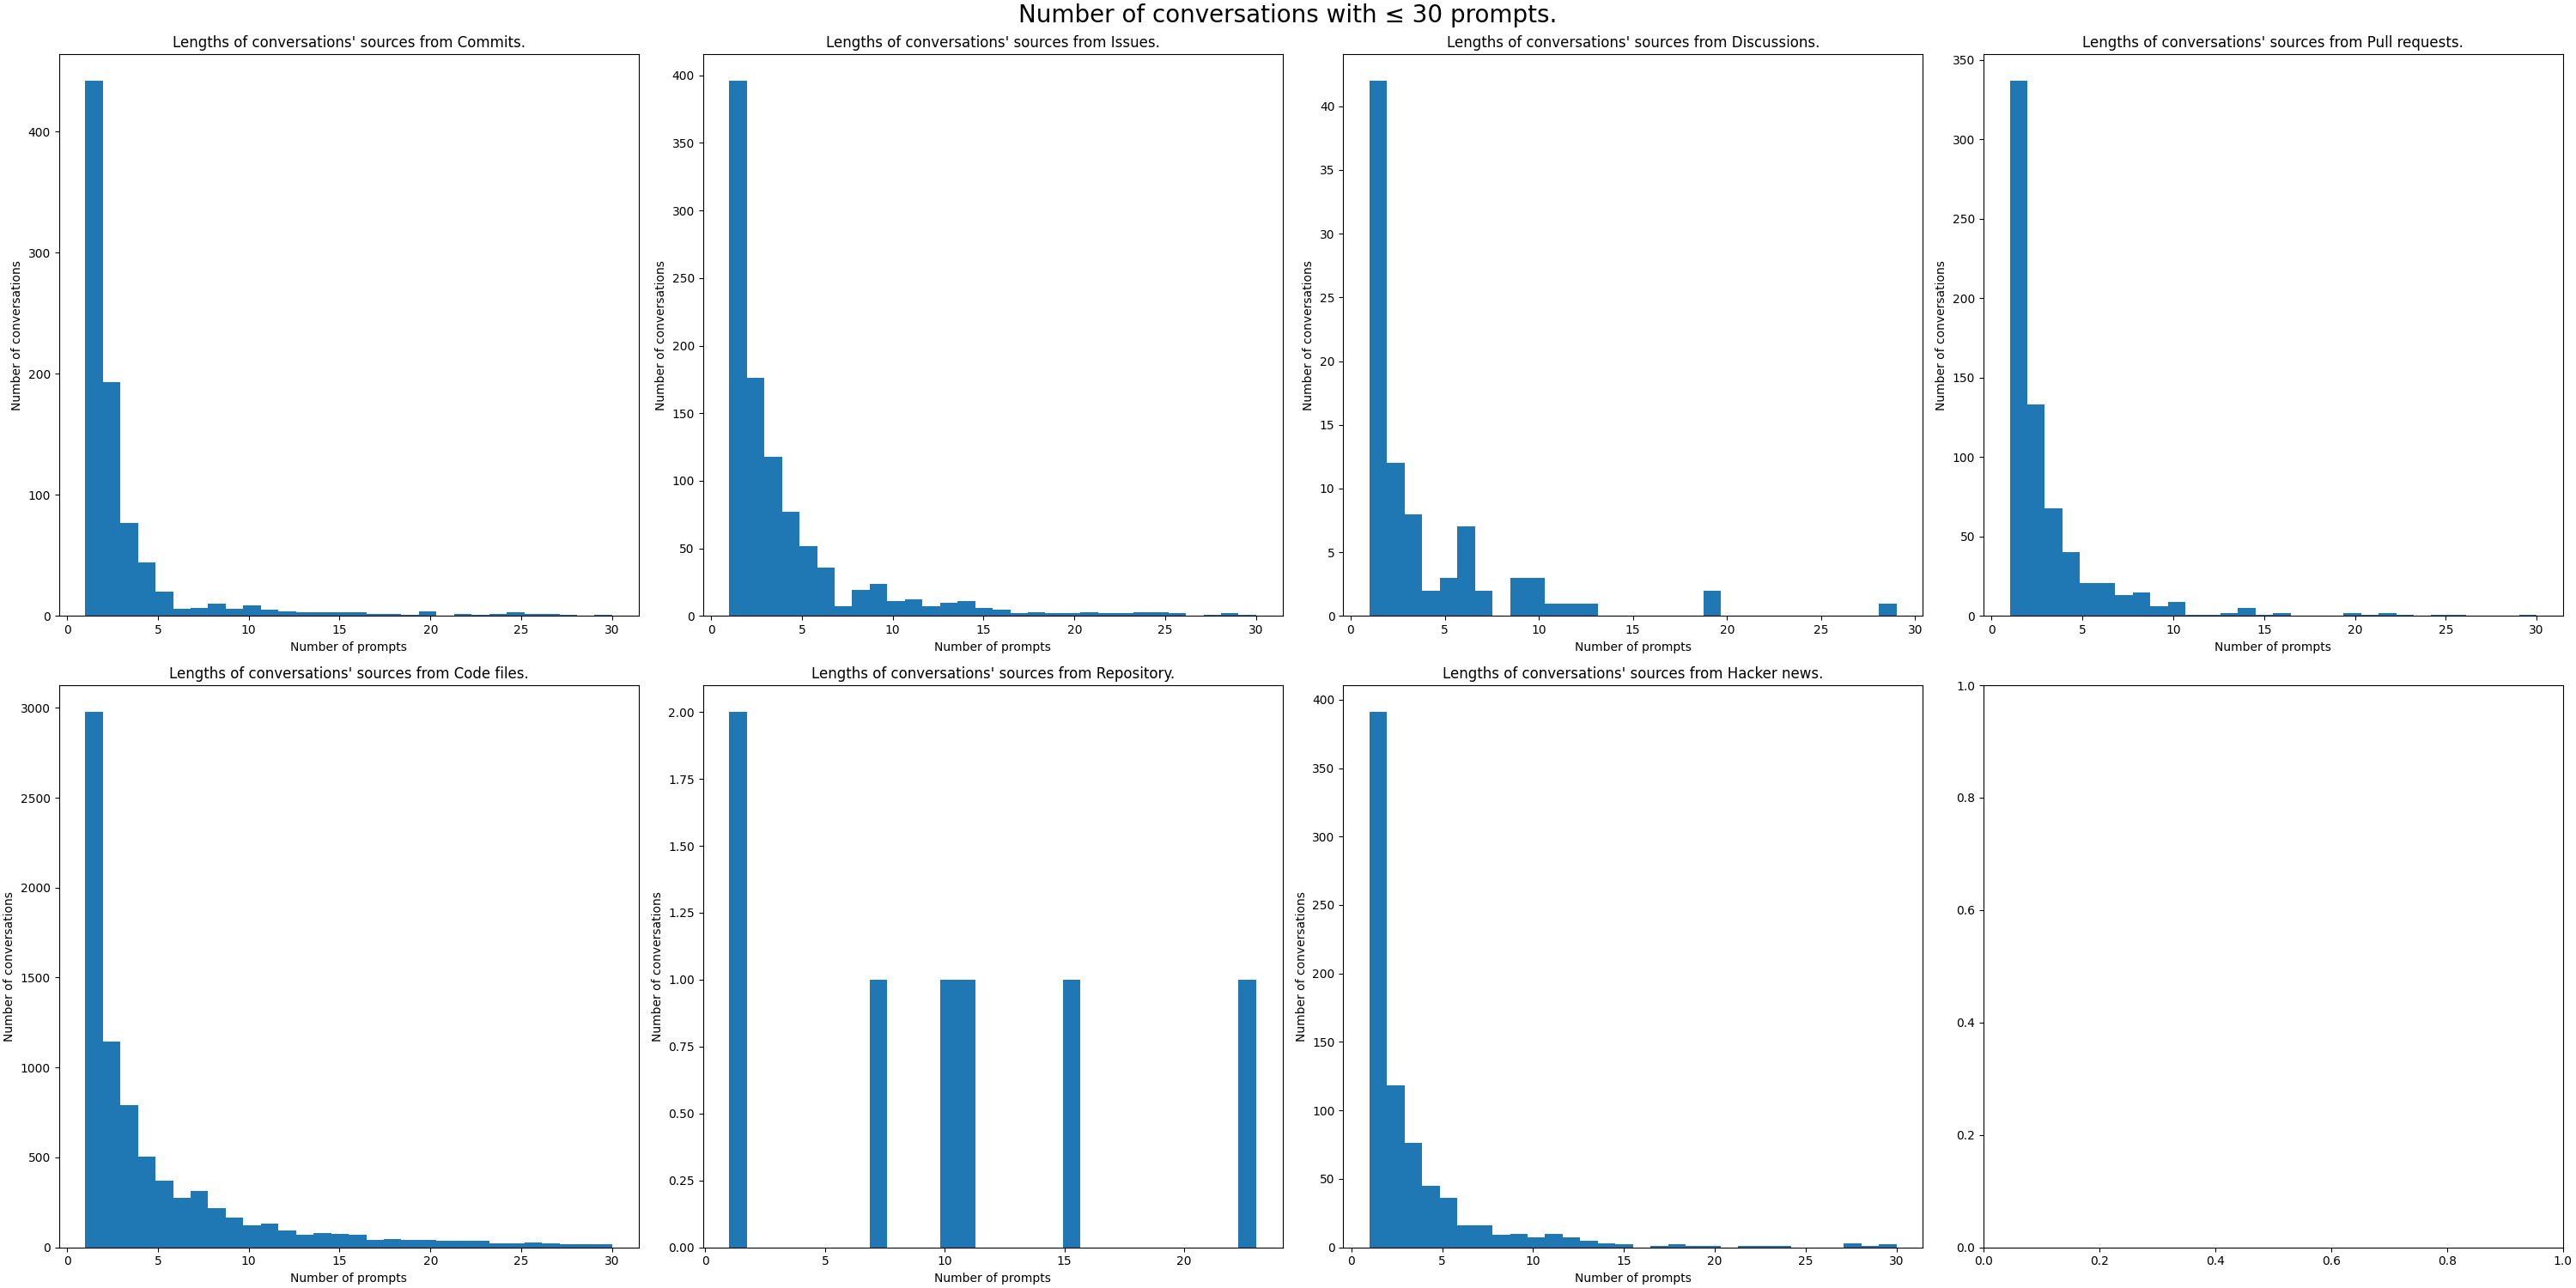
\includegraphics[width=\textwidth]{imgs/conv-per-prompt-nr.png}
    \caption{Lengths of conversations in histogram gathered from different sources.}
    \label{fig:conv-per-prompt}
\end{figure}

\subsubsection{Long conversations contents}
To understand the reasons behind unusually long conversations, we manually reviewed conversations that exceeded a predefined length threshold. The most common patterns are summarised below:

\begin{itemize}
    \item \textbf{Pasted content:} Users split large texts (e.g., code files, articles, books) into multiple prompts due to the prompt's character limits.
    \item \textbf{Iterative debugging:} Users refined requests or sought help with errors after initial code responses did not meet their expectations.
    \item \textbf{Programming assistance:} Users guided \acrshort{gpt} through multi-step coding tasks, testing and iterating on output.
    \item \textbf{Mentorship:} Users shared their own code for feedback, explanations, or improvement suggestions.
    \item \textbf{General discussion:} Some conversations focused on non-programming topics such as advice, opinions, or general discussions.
\end{itemize}

\subsubsection{Average symbol/word count per prompt}
The average number of symbols per prompt varied across sources, as shown in Figure~\ref{fig:symbols-per-prompt}. The \textit{x}-axis represents the prompt position within a conversation, while the \textit{y}-axis shows the average symbol count for that position. Since longer conversations are less common, later prompt positions often reflect fewer data points --- leading to the prompt average pattern changes that can be visibly observed in the conversations sourced from GitHub code files or Hacker News. Across majority of the sources, initial prompts typically have higher symbol counts, as they often introduce the problem in detail.

\begin{figure}[H]
    \centering
    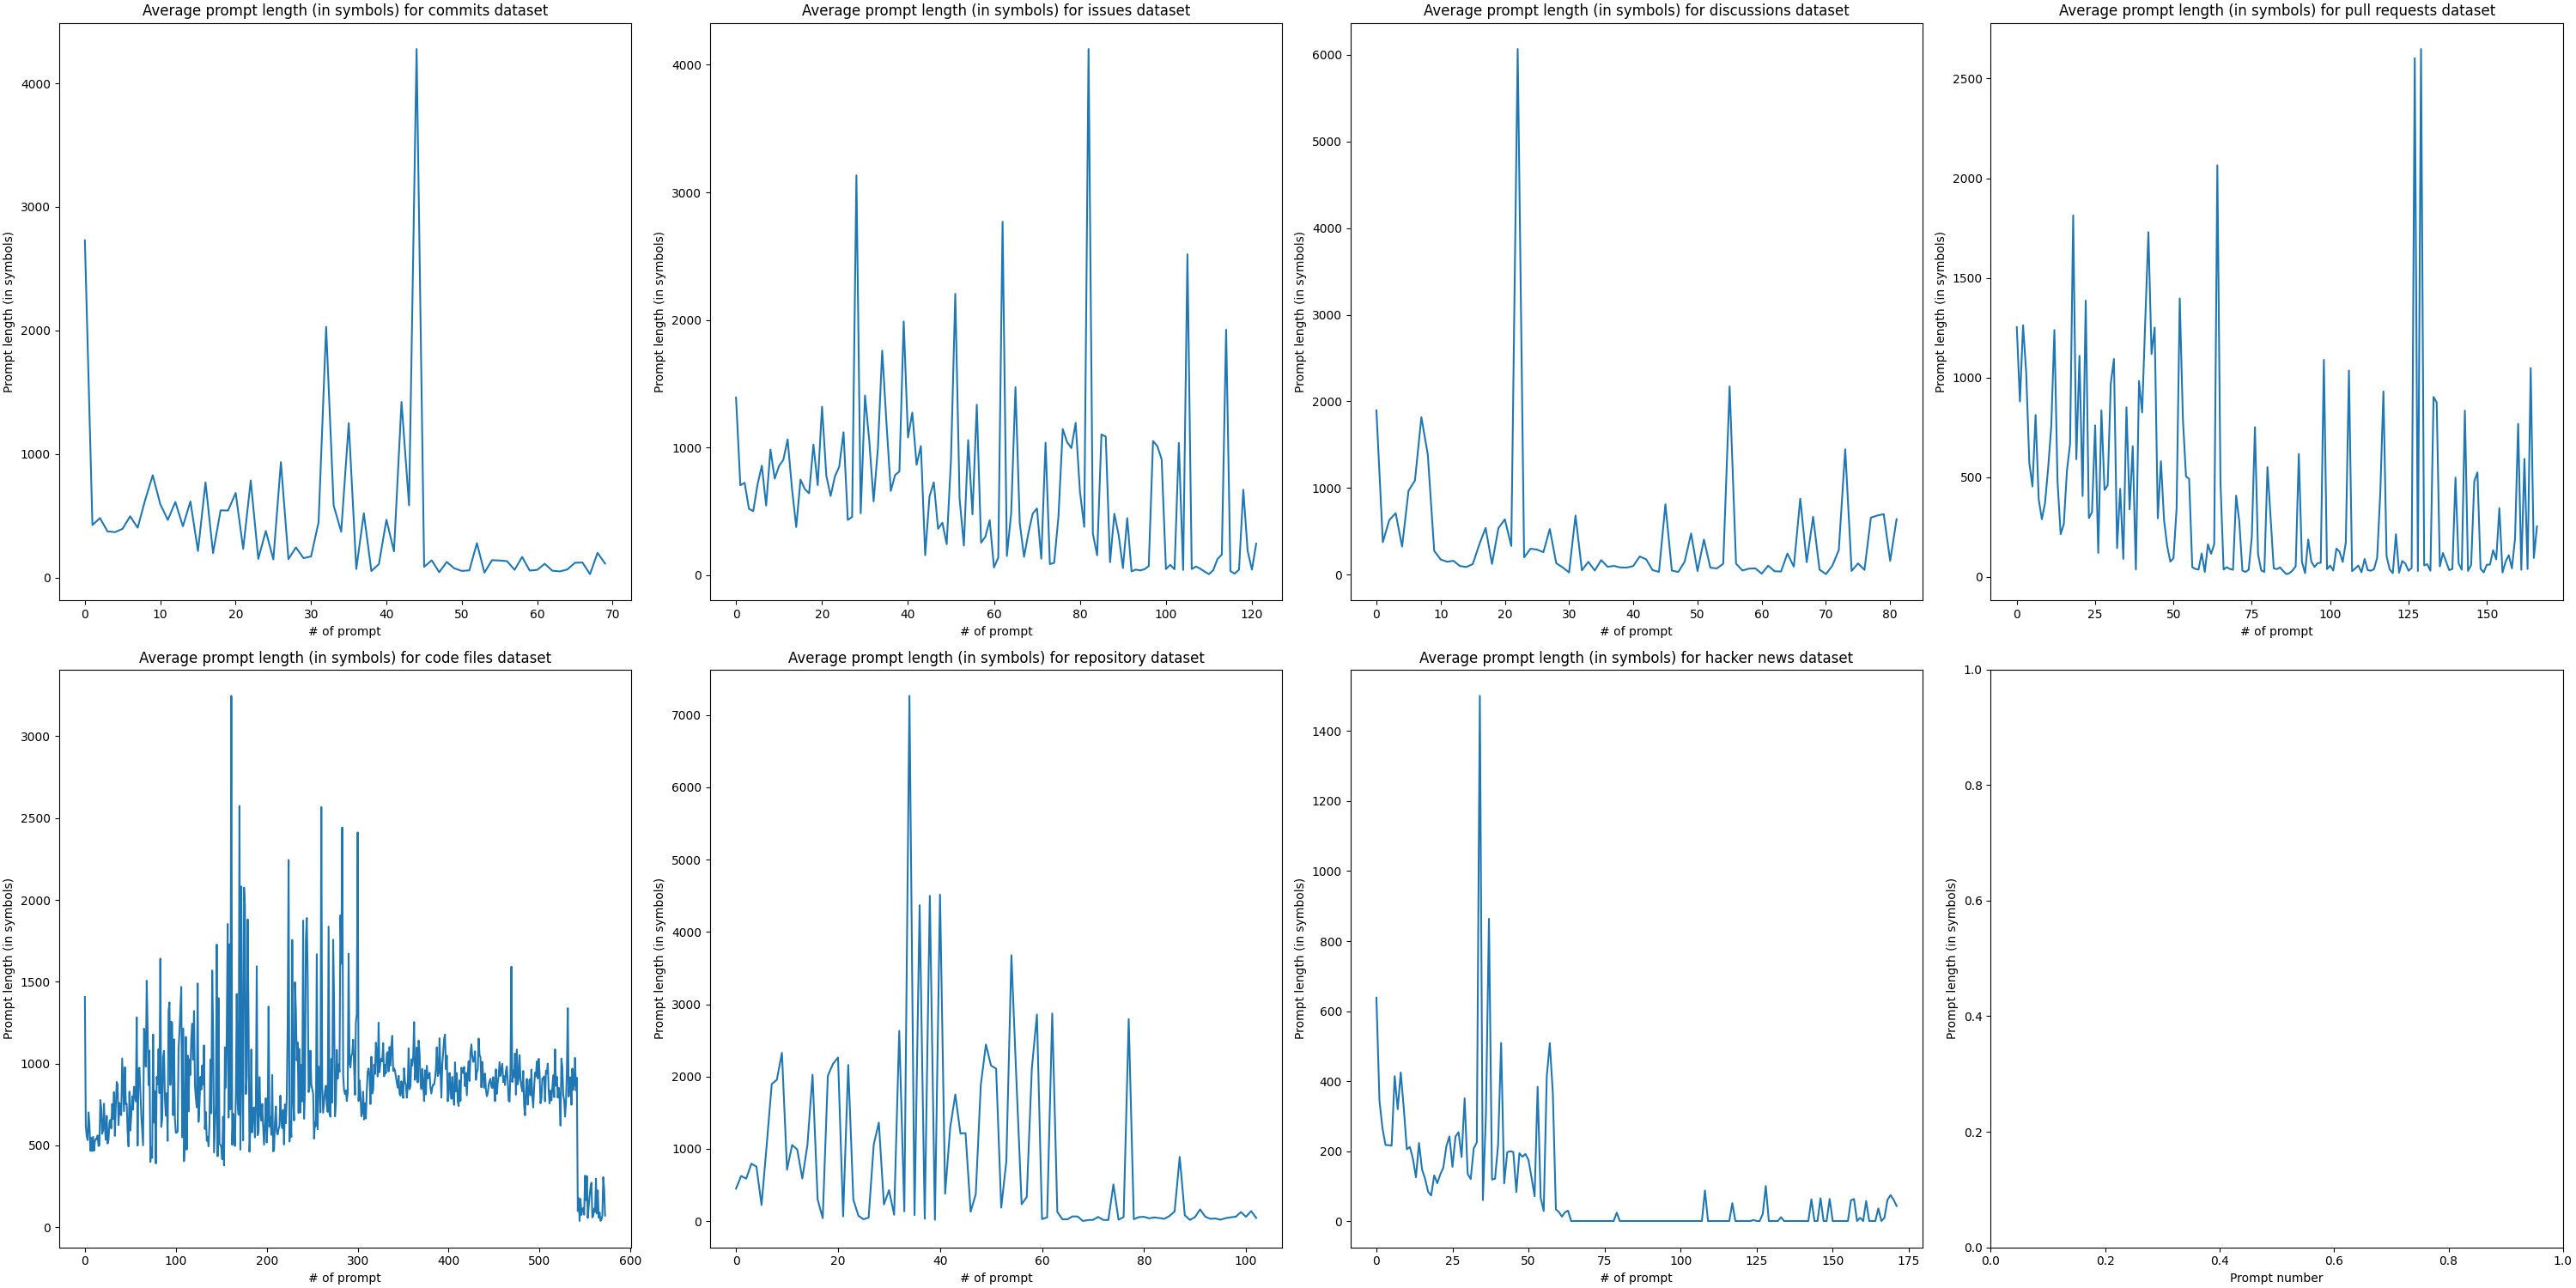
\includegraphics[width=\textwidth]{imgs/symbols-per-prompt.png}
    \caption{Average symbol count per prompt number for all conversation sources after code lines were removed.}
    \label{fig:symbols-per-prompt}
\end{figure}

To identify outliers, we defined dataset-specific cut-off thresholds set at two-thirds of the maximum observed average. Conversations containing prompts exceeding these thresholds were saved for further analysis.

\subsubsection{Long prompt contents}
Conversations containing unusually long prompts were saved and manually reviewed to understand their content. We identified several common reasons for the prompt length:
\begin{itemize}
    \item \textbf{Pasted external content:} Users copied large texts from sources such as scientific articles, GitHub issues, or documentation, often asking for summaries, explanations, or audience-specific rewrites.
    \item \textbf{Code-related debugging:} Prompts included error messages, undocumented code, or comments not flagged as code, with users seeking help with debugging or improvement.
    \item \textbf{Detailed problem descriptions: } Some users provided extensive background to frame their query, including:
    \begin{itemize}
        \item Highly specific requests or detailed issue descriptions;
        \item Roleplay-style prompts (e.g., asking \gls{gpt} to act as a mentor or expert);
        \item Contextual or background information;
        \item Multiple follow-up questions or clarifications;
        \item Previously attempted (but unsuccessful) solutions;
        \item Long URLs or resource links;
        \item Lists of requirements or instructions;
        \item Desired output examples or target functionality.
    \end{itemize}
\end{itemize}
